% Journal version (target: Science and Medicine in Football; fallback: JQAS / IJCSS).
% Every number comes from docs/results/*.md (rows 1-25 of docs/PAPER_V2_NOTES.md); figures from
% paper/journal/make_journal_figures.py. Check the journal's author guidelines (word limit, abstract format,
% reference style, figure/table limits, title page and anonymisation) before submission.
\documentclass[11pt]{article}

\usepackage[T1]{fontenc}
\usepackage[utf8]{inputenc}
\usepackage[margin=2.5cm]{geometry}
\usepackage{setspace}
\usepackage{lineno}
\usepackage{graphicx}
\usepackage{booktabs}
\usepackage{amsmath}
\usepackage{xcolor}
\usepackage[round,authoryear]{natbib}
\usepackage{hyperref}
\newcommand{\todo}[1]{\textcolor{red}{[TODO: #1]}}

\title{How much can you trust broadcast pressing data? Visibility bias in team pressing metrics, its drivers, and a
correction validated on real broadcast video}
\author{Varun Inamdar\\
Vishwakarma University, Pune, India\\
\texttt{vninamdar03@gmail.com}}
\date{}

\begin{document}
\maketitle
\doublespacing
\linenumbers

\begin{abstract}
Tracking data derived from broadcast video is widely available, but the main camera shows only about 14 of the 22
players at a time. We quantified how this partial view biases pressing metrics and how to correct it. Using full
optical tracking of 10 professional matches from two providers (14 teams), we hid every player that a broadcast camera
would not show and recomputed pressing intensity. The camera was fitted to the on-pitch footprints of 20 real
broadcasts and validated on held-out matches (87.1\% per-player agreement; visible players reproduced exactly).
Averaged over 20 stadium cameras, broadcast tracking undercounted a team's active pressers by 22.6\% (95\% CI 19.8 to
25.2) in one dataset and 20.2\% (17.1 to 23.2) in the other; every one of the 14 teams was undercounted (18--28\%).
The undercount was almost fully explained by the number of visible players ($r = 0.98$; about 4 percentage points per
player), whereas pressure on the ball carrier was nearly unbiased unless the camera lagged. A correction based on the
number of visible players reduced the mean absolute error from 21.9\% to 3.0\% on broadcasts whose stadium camera and
match were both held out, and to 4.7\% on cameras fitted to a second league within the fitted visibility range. On
real broadcast video, an open pipeline counted visible players to within about half a player after calibration on
two independent datasets, keeping the corrected error at 3.0--3.6\% over a whole match. Live main-camera footage made up 64\% of 196
fully labelled broadcasts, so close-ups must be filtered out before counting. Team-wide pressing metrics from
broadcast data should therefore be corrected, or compared only between broadcasts with similar camera framing.
\end{abstract}

\noindent\textbf{Keywords:} football; broadcast tracking; pressing; measurement bias; performance analysis;
computer vision

% =============================================================================================
\section{Introduction}

Pressing, how intensely a team without the ball closes down the opponent, is one of the most discussed tactical
concepts in modern football. Quantifying it requires the positions of all players. Full optical tracking provides
them, but most clubs, analysts and researchers cannot access it. Tracking data extracted from broadcast video is a much
cheaper alternative. It is increasingly offered commercially and studied academically
\citep{somers2024gsr,smf2025broadcast}. Its limitation is structural: the broadcast camera follows the action, so
players far from the ball are often off screen.

For spatial metrics such as pitch control, this partial view causes large errors in the hidden areas of the pitch
\citep{offscreen2026}, and several methods impute off-screen players
\citep{omidshafiei2022graphimputer,rsos2025continuous,offscreen2026}. Comparing broadcast-derived with official
tracking, \citet{smf2025broadcast} found that less than half of the players' activity is visible on TV broadcasts.
They concluded that some tactical analyses remain reliable, while physical metrics are more affected. For pressing
metrics, the size of the bias, what drives it and how certain we can be about it have not been measured. Pressing
involves the defenders near the ball and also those covering passing lanes further away. It is therefore not obvious
whether a ball-following camera biases it at all.

This study addressed five questions. (1) How large is the visibility bias in pressing metrics, and how certain is it?
(2) Is it driven by particular teams, matches or stadium cameras? (3) Which measurable properties of a broadcast drive
it? (4) Can it be corrected, also for broadcasts filmed in another league? (5) Does the correction work on real
broadcast video, where its input must be measured by computer vision and replays and close-ups interrupt the main
camera?

% =============================================================================================
\section{Methods}

\subsection{Data}

\textbf{Ground-truth tracking.} The IDSSE open dataset \citep{bassek2025idsse} (CC-BY 4.0) contains optical tracking
of all 22 players and the ball at 25\,Hz for 7 matches of the 2022/23 Bundesliga and 2.~Bundesliga, with possession
information (552{,}294 ball-in-play frames). As a second, independent provider we used the 3 Metrica Sports sample
games \citep{metrica_sample} (25\,Hz, all players). Their possession and ball-in-play status were reconstructed from
the accompanying event files. Together the ground truth covers 10 matches and 14 teams. One team, Fortuna
D\"usseldorf, appears in 5 of the 7 IDSSE matches; Section~\ref{sec:teams} tests whether it drives the results. All
tracking data were loaded with kloppy \citep{kloppy}.

\textbf{Real broadcast footprints.} The SkillCorner open data \citep{skillcorner_opendata} (MIT licence) contains
broadcast tracking of 20 A-League 2024/25 matches at 10\,Hz. For every frame it gives the four corners of the camera
image projected onto the pitch, and for every player whether they were detected on screen. These data were used only
to fit and validate the camera model (375{,}357 frames).

\textbf{Broadcast video.} SoccerNet-GSR \citep{somers2024gsr} (GPL-3.0) contains 30-second main-camera clips from the
Swiss Super League (25\,Hz, 1920$\times$1080). For every frame it labels each person's box, role, team, jersey number
and pitch position. We trained on the 57 training clips, tuned on half of the 58 validation clips and report on the
other half and on the 49 test clips. As a fully independent test of the visible-player count we used the 30 labelled
football clips of SportsMOT \citep{cui2023sportsmot} (CC BY-NC 4.0; 20{,}171 frames, 1280$\times$720). They come
from other broadcasts, and only players on the pitch are labelled. The labelled clips of SoccerNet-Tracking were not
used: all 106 are also SoccerNet-GSR clips.

\textbf{Broadcast composition.} The SoccerNet-v2 camera-shot labels \citep{deliege2021soccernetv2} mark every camera
change in 500 full broadcasts (2014--2017; Premier League, La Liga, Serie A, Bundesliga, Ligue 1 and Champions
League). We used them to measure how much of a broadcast is not the live main camera. No video frames are reproduced
in this article.

\subsection{Pressing metrics}
For each frame with a ball carrier we computed the matrix $P$ of interception probabilities between defenders and
attackers \citep{bekkers2025pressing}, using \texttt{unravelsports} \citep{unravelsports} with a speed threshold of
2\,m/s. We report two summaries per frame. \emph{Pressure on the ball carrier}, $1 - \prod_i (1 - P_{i,c})$ over
defenders $i$ for carrier $c$, is a local metric. The number of \emph{active pressers}, defenders whose largest
probability exceeds 0.5, is a team-wide metric. Frames without a ball carrier in the possessing team were dropped:
0.06--0.2\% per IDSSE match and 6.8\% for Metrica, whose possession comes from hand-annotated events.

\subsection{A broadcast camera fitted to real footage}
The main camera was modelled as a fixed point $(c_x, c_y)$ behind the near touchline. A player at bearing $\theta$
from the camera is visible if $|\theta - \phi_t| \le \alpha_t/2$ and their depth along the viewing direction exceeds
the bottom image edge $\nu_t$:
\begin{align}
\phi_t &= \mathrm{EMA}_{\lambda}\!\left(g_b\,\theta^{\text{ball}}_t + g_p\,\bar\theta^{\text{players}}_t + o\right),\\
\alpha_t &= \mathrm{clip}\!\left(a_0 + a_1 d^{\text{ball}}_t + a_2\, s^{\text{players}}_t\right),\qquad
\nu_t = n_0 + n_1 d^{\text{ball}}_t.
\end{align}
Here $\phi$ is the pan and $\alpha$ the horizontal field of view. $d^{\text{ball}}$ is the ball's distance from the
camera, $\bar\theta^{\text{players}}$ and $s^{\text{players}}$ are the mean and standard deviation of the players'
bearings, and $\lambda$ is an exponential lag.

In every SkillCorner frame, the left and right image edges are rays from the camera's ground position; their
intersection locates the camera (median per match). Pan and field of view follow from the bearings of the far image
corners, and the bottom edge from the near corners. The coefficients were fitted by least squares and $\lambda$ by
grid search (0--1\,s). One shared camera was fitted on 10 matches and tested on the other 10 against the per-player
detection flags. To capture differences between stadiums we also fitted one camera per match (20 stadium cameras).
The commonly assumed baseline is a full-width window of fixed length centred on the ball.

\subsection{Simulating the broadcast view and estimating the bias}
Given full tracking and a camera, we removed every player outside the camera's view and recomputed the metrics on the
remaining players. The ball and the ball carrier were always kept, and a frame with no visible defender counted as
zero pressure. The bias of a metric is the relative difference between a team's out-of-possession mean with and
without hiding. Each stadium camera was applied to each ground-truth match, giving 400 team-broadcasts
(20 cameras $\times$ 10 matches $\times$ 2 teams).

\subsection{Correction}
Because the bias of active pressers was nearly linear in the number of visible players (Section~\ref{sec:drivers}),
we corrected a broadcast's value by fitting $\text{bias} = k \cdot \text{visible} + b$ across broadcasts and dividing
by $1 + \text{bias}$. The correction was evaluated strictly. For every team-broadcast, the line was fitted without its
stadium camera and without its match. In a stricter variant, every match of its pressing team was also left out.

\subsection{Robustness and generalisation}
\label{sec:robust-methods}
\textbf{Teams.} We report the bias per team, a team-balanced mean (every team weighs the same) with an interval from
resampling teams, and leave-one-team-out estimates. We also estimated the extra bias of the most frequent team at
equal visibility, from the least-squares model $\text{bias} = a + b\cdot\text{visible} + c\cdot[\text{team}]$ with a
match-level bootstrap.

\textbf{A second league.} SoccerNet-GSR gives no camera parameters. However, each person's labelled pitch position
is an exact projection of the bottom of their box. A homography fitted to these positions per frame therefore maps the
image corners onto the pitch, giving the same footprints as SkillCorner. We fitted the camera model in this way to 6
Swiss Super League broadcasts. Off-screen players are unknown in this data, so the pan followed the ball only. The
Swiss cameras were applied to all 10 ground-truth matches (120 team-broadcasts). These broadcasts were corrected with
the line fitted on the A-League cameras, leaving out each broadcast's match.

\subsection{Measuring visible players on real video}
The correction needs one number per broadcast: the mean number of visible players per frame (both teams and the
goalkeepers, no referees). We measured it with an open pipeline.
\begin{itemize}
\item \emph{Detection.} An RF-DETR Medium detector \citep{rfdetr} fine-tuned on SoccerNet-GSR (95.8\% recall, 95.5\%
precision for people on validation).
\item \emph{Tracking.} OC-SORT \citep{cao2023ocsort} with camera-motion compensation \citep{trackers}.
\item \emph{Teams and roles.} Teams from per-clip $k$-means on shirt colour. Tracks that fit neither team are
goalkeepers inside a penalty area and referees elsewhere.
\item \emph{Pitch calibration.} A ResNet-34 \citep{he2016resnet} pitch-landmark network with a RANSAC homography.
\item \emph{Jersey numbers.} A fine-tuned scene-text recogniser (PARSeq; \citealp{bautista2022parseq}).
\end{itemize}
The count of visible players uses the tracked people whose role is player or goalkeeper. It does not need a
homography. A linear calibration ($\text{labels} \approx a\cdot\text{count} + b$) was fitted on the SoccerNet-GSR
tuning clips only and applied unchanged to all other data.

The counting error was propagated into the correction. For each team-broadcast we added count errors drawn from the
held-out clips to its true visible-player mean (500 draws). A broadcast is a whole match, about 180 clips, so we
averaged 180 clip errors per draw. As a worst case we also used the error of a single clip.

\textbf{Replays and close-ups.} Non-main-camera frames must not enter the count. A main-camera filter removes shots
with little grass ($<0.2$ of the frame) or very large people (median box over 300\,px). Shot boundaries come from
colour-histogram cuts, and each shot is kept or dropped as a whole. From the SoccerNet-v2 labels we measured the
share of broadcast time per camera type. On 203 games we verified that a label describes the shot ending at its
timestamp: at shots on target and goals, 99\% of labels read this way are the live main camera. We then derived how
many non-main frames the filter may let through before the correction moves by more than 1 percentage point.

\subsection{Statistics}
Frames 40\,ms apart are strongly dependent, so we used a block bootstrap with 60\,s blocks within each team-match.
Across stadium cameras, a three-level bootstrap resampled cameras, matches (both teams together) and blocks
(2{,}000 replicates, 95\% percentile intervals). For the stadium-camera runs, metrics were evaluated every 0.2\,s
while the camera followed every frame. This changed the bias by less than 0.1 percentage points (checked on one full
match). Counting errors on video are reported with intervals from resampling whole clips.

% =============================================================================================
\section{Results}

\subsection{The fitted broadcast camera}

\begin{figure}[t]
\centering
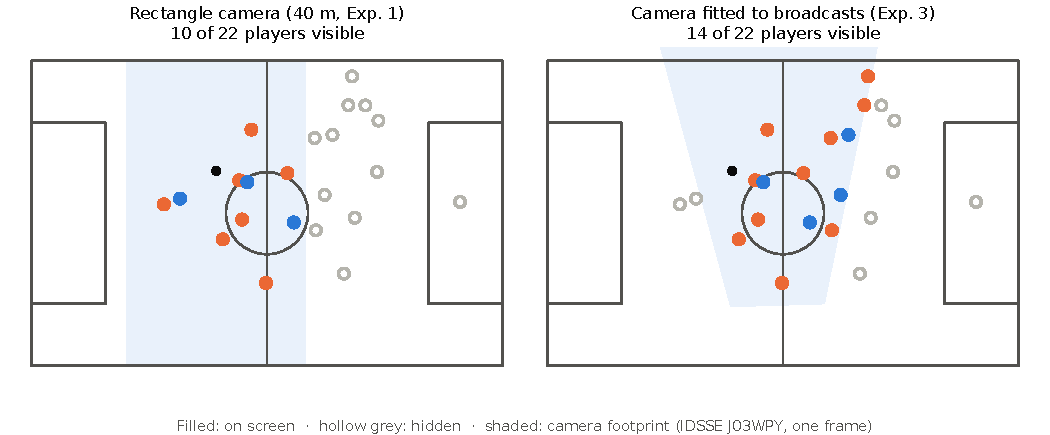
\includegraphics[width=\textwidth]{figures/fig1_cameras.pdf}
\caption{The same frame seen by the commonly assumed rectangle camera (left) and the camera fitted to real broadcasts
(right). The fitted camera stands behind the near touchline: its footprint widens towards the far side and cuts off
players close to the camera.}
\label{fig:cameras}
\end{figure}

The fitted camera stood on the halfway line, 57--97\,m from the pitch centre depending on the stadium. Its pan
followed the ball and the players' centre with similar weights ($g_b = 0.57$, $g_p = 0.56$; $R^2 = 0.97$). The shared
camera showed no measurable lag. The median field of view was 27$^\circ$ (19--40$^\circ$); it narrowed when play was
far away and widened when players were spread out (Figure~\ref{fig:cameras}). On 10 held-out matches the fitted camera
predicted which players were on screen with 87.1\% agreement, against 82.9\% for a 40\,m rectangle and a 96.8\% upper
bound from the real footprint. It beat the rectangle on every held-out match and reproduced the mean number of visible
players exactly (14.65; Table~\ref{tab:validation}). A camera following only the ball underestimated visibility
(13.30 players), showing that camera operators frame the players, not only the ball.

\begin{table}[t]
\centering
\caption{Which players are on screen? Agreement of each camera model with SkillCorner's per-player detection flags on
10 held-out matches.}
\label{tab:validation}
\begin{tabular}{lcc}
\toprule
Camera model & Agreement & Visible players per frame \\
\midrule
Real footprint (upper bound) & 96.8\% & -- \\
\textbf{Fitted camera} & \textbf{87.1\%} & \textbf{14.65} \\
Rectangle, 40\,m & 82.9\% & 15.76 \\
Rectangle, 32\,m with assumed lag, perspective and zoom & 82.2\% & 15.29 \\
Fitted camera following the ball only & 82.0\% & 13.30 \\
\midrule
Real broadcast & -- & 14.65 \\
\bottomrule
\end{tabular}
\end{table}

\subsection{Visibility bias in pressing metrics}

\begin{table}[t]
\centering
\caption{Relative bias of pressing metrics under different cameras (negative = undercount), with 95\% bootstrap
intervals. The stadium-camera interval includes camera, match and within-match variation.}
\label{tab:bias}
\small
\begin{tabular}{llccc}
\toprule
Data & Camera & Visible & Pressure on carrier & Active pressers \\
\midrule
IDSSE (7) & Rectangle 40\,m & 14.5 & $-0.1\%$ [$-0.2$, $-0.1$] & $-20.3\%$ [$-22.7$, $-17.9$] \\
IDSSE (7) & Rectangle 40\,m, assumed 0.5\,s lag & 14.3 & $-4.1\%$ [$-4.6$, $-3.7$] & $-24.1\%$ [$-26.5$, $-21.9$] \\
IDSSE (7) & Fitted shared camera & 13.8 & $-0.5\%$ [$-0.7$, $-0.4$] & $-21.4\%$ [$-23.8$, $-19.1$] \\
IDSSE (7) & \textbf{20 stadium cameras} & 12.1--16.0 & $\mathbf{-1.7\%}$ [$-2.2$, $-1.2$] & $\mathbf{-22.6\%}$ [$-25.2$, $-19.8$] \\
Metrica (3) & \textbf{20 stadium cameras} & 12.7--16.6 & $\mathbf{-1.8\%}$ [$-2.3$, $-1.3$] & $\mathbf{-20.2\%}$ [$-23.2$, $-17.1$] \\
\bottomrule
\end{tabular}
\end{table}

With every camera model, broadcast tracking undercounted a team's active pressers by about one fifth
(Table~\ref{tab:bias}). Averaged over the 20 stadium cameras, the undercount was 22.6\% for IDSSE and 20.2\% for
Metrica. Pressure on the ball carrier was much less affected ($-0.5\%$ to $-1.8\%$). The stadium camera alone
contributed as much uncertainty as the sample of matches (IDSSE, active pressers: camera only [$-24.3$, $-20.6$];
matches and blocks only [$-24.4$, $-20.6$]). The same camera showed about one more player on Metrica than on IDSSE.
At equal visibility the two providers agreed: at 14.5 visible players, the undercount of active pressers was 19.6\% in
both datasets.

\subsection{What drives the bias}
\label{sec:drivers}

\begin{figure}[t]
\centering
\begin{minipage}{0.49\textwidth}\centering
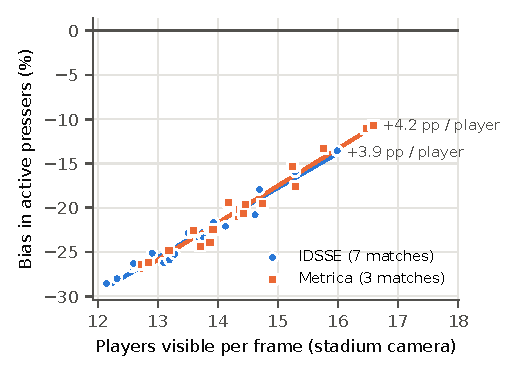
\includegraphics[width=\linewidth]{figures/fig2_visibility.pdf}
\end{minipage}\hfill
\begin{minipage}{0.49\textwidth}\centering
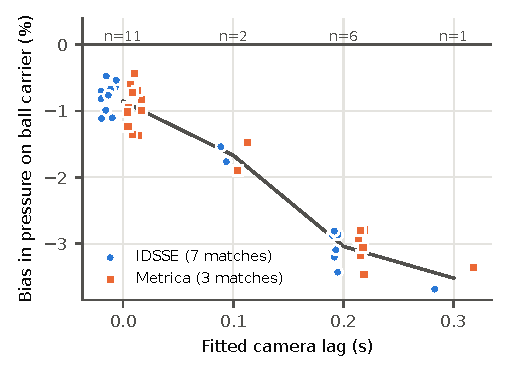
\includegraphics[width=\linewidth]{figures/fig3_lag.pdf}
\end{minipage}
\caption{One point per stadium camera and dataset. Left: the undercount of active pressers shrinks by about
4 percentage points per additional visible player ($r = 0.98$). Right: the bias in pressure on the ball carrier grows
with the camera's fitted lag; $n$ = number of stadium cameras per lag value.}
\label{fig:drivers}
\end{figure}

Across stadium cameras, the bias was almost fully explained by two properties of the broadcast
(Figure~\ref{fig:drivers}). For active pressers it was the \textbf{number of visible players}. Broadcasts that framed
the whole group (15--16.6 players visible) missed 11--14\%, and tight framing (about 12 visible) missed up to 29\%
($r = 0.98$ in both datasets; 3.9 and 4.2 percentage points per player). For pressure on the ball carrier it was
\textbf{camera lag}. The 11 stadium cameras without measurable lag gave $-0.9\%$; 0.1\,s of lag gave $-1.7\%$, 0.2\,s
$-3.0\%$ and 0.3\,s $-3.5\%$ ($r = -0.97$ across cameras). When the camera trails the ball, defenders closing down the
carrier enter the picture late.

\subsection{Correcting the bias}
\label{sec:correction}
Over the 400 team-broadcasts, the pooled slope was 4.1 percentage points per visible player. With the stadium camera
and the match held out, the correction reduced the mean absolute error in active pressers from 21.9\% to
\textbf{3.0\%}, and 95\% of broadcasts were within $\pm 7.0\%$. With the pressing team also unseen, the error was
3.2\% (95th percentile 7.6\%). Per match, the corrected error ranged from 1.5\% to 4.9\%.

\subsection{Robustness to teams}
\label{sec:teams}
Every one of the 14 teams was undercounted, by 17.8--27.9\%. The team-balanced mean was $-22.1\%$
[$-23.8$, $-20.4$] for IDSSE and $-20.8\%$ [$-22.5$, $-19.0$] for Metrica. Leaving out all matches of any one IDSSE
team gave mean biases between $-19.5\%$ (without Fortuna D\"usseldorf, 2 matches left) and $-23.2\%$, with slopes of
3.9--4.2 percentage points per player. At equal visibility, Fortuna's extra bias was $-1.9$ percentage points
[$-5.3$, $+1.5$], so it did not differ from the other teams.

\subsection{A second league's cameras}
\label{sec:league}

\begin{figure}[t]
\centering
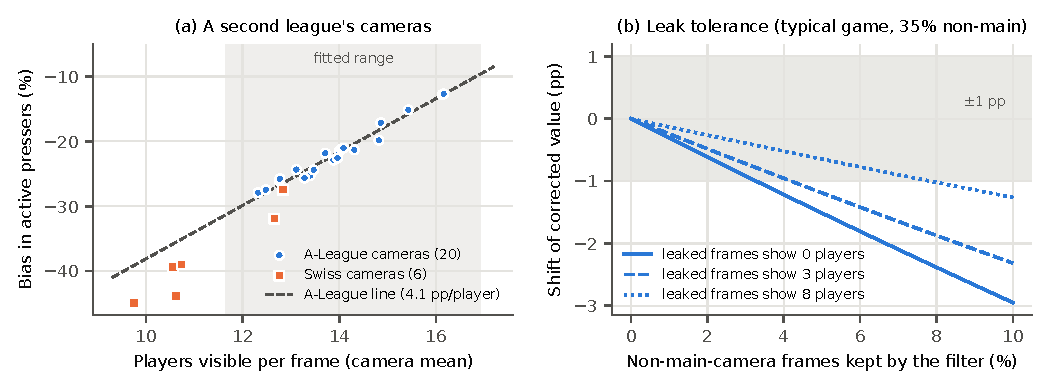
\includegraphics[width=\textwidth]{figures/fig5_generalisation.pdf}
\caption{(a) Bias in active pressers for cameras fitted to six Swiss Super League broadcasts (squares; mean over the
10 ground-truth matches) against the A-League cameras and their correction line. The shaded band is the visibility
range the line was fitted on. (b) How far the corrected value moves when the main-camera filter keeps a share of the
non-main-camera frames, for a typical broadcast (35\% non-main) with 14 visible players on main-camera frames.}
\label{fig:generalisation}
\end{figure}

The six Swiss cameras stood 51--66\,m from the pitch centre, with median fields of view of 24--34$^\circ$. Following
only the ball, they showed 9.8--12.8 players. That is fewer than the 11.5--16.0 players visible in the real Swiss
broadcasts, because the players' influence on the pan could not be fitted. Their bias in active pressers was
27--45\%, and it fell more steeply with visibility than for the A-League cameras (5.1 against 4.1 percentage points
per player; Figure~\ref{fig:generalisation}a). With the A-League line, the corrected mean absolute error was
\textbf{4.7\%} for broadcasts within the visibility range the line was fitted on ($\ge 11.7$ players). Below that
range it was 8.8\%, an under-correction that a quadratic fit did not remove. Fitting the line on both leagues
together brought the error to 4.6\% (95th percentile 11.5\%).

\subsection{From real broadcast video}

\begin{table}[t]
\centering
\caption{End-to-end game state on SoccerNet-GSR test (49 clips), scored with the official evaluator. GS-HOTA matches
a prediction to a labelled person only within 5\,m and with the same role, team and jersey number
\citep{luiten2021hota}. The position-only score ignores the attributes and uses our implementation of the same
similarity.}
\label{tab:gsr}
\begin{tabular}{lcc}
\toprule
Pipeline & GS-HOTA & Position only \\
\midrule
SoccerNet-GSR baseline \citep{somers2024gsr} & 22.3 & 42.7 \\
Ours, no jersey numbers & 24.0 & 62.3 \\
Ours, with jersey numbers & \textbf{39.8} & 62.3 \\
\bottomrule
\end{tabular}
\end{table}

\textbf{Pipeline.} The pipeline reconstructed the game state well above the public baseline (Table~\ref{tab:gsr}).
The relevant output here, however, is the count of visible players.

\begin{table}[t]
\centering
\caption{Counting visible players on real video: mean error (pipeline minus labels, players per frame) with 95\%
intervals from resampling clips, error of 30-second clip means, and correlation of clip means. The calibration was
fitted on SoccerNet-GSR tuning clips only.}
\label{tab:count}
\small
\begin{tabular}{llccc}
\toprule
Data & Count & Mean error [95\% CI] & Clip MAE & Clip $r$ \\
\midrule
SoccerNet-GSR, held-out valid (29 clips) & raw & $-1.05$ [$-1.41$, $-0.75$] & 1.07 & 0.95 \\
SoccerNet-GSR, held-out valid (29 clips) & calibrated & $-0.32$ [$-0.68$, $-0.01$] & 0.67 & 0.95 \\
SportsMOT, independent (30 clips) & raw & $-0.26$ [$-0.54$, $-0.01$] & 0.70 & 0.90 \\
SportsMOT, independent (30 clips) & calibrated & $+0.53$ [$+0.26$, $+0.79$] & 0.78 & 0.90 \\
\bottomrule
\end{tabular}
\end{table}

\textbf{Counting visible players.} On SoccerNet-GSR the pipeline undercounted by about one player, and the calibration
removed this bias (Table~\ref{tab:count}). The players it missed were small or hidden in groups. On the independent
SportsMOT clips the raw count was already close ($-0.26$ players), so the calibration over-corrected ($+0.53$). Adding
SportsMOT's own training clips to the calibration barely changed this ($+0.42$). The calibration offset therefore
depends on the dataset. After calibration, though, the count was within about half a player on both datasets
($-0.32$ and $+0.53$), and the clip means followed the labels closely ($r = 0.90$--$0.95$).

\begin{figure}[t]
\centering
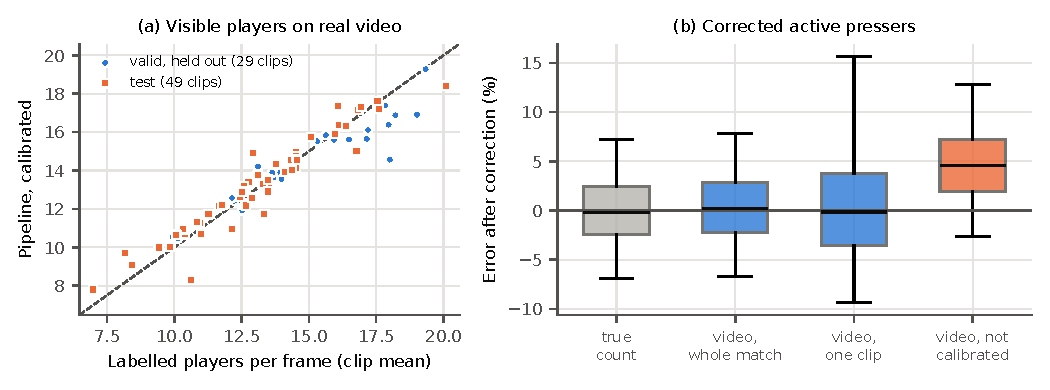
\includegraphics[width=\textwidth]{figures/fig4_real_video.pdf}
\caption{(a) Visible players per 30-second clip: calibrated pipeline count against labels (SoccerNet-GSR, held-out
validation and test). (b) Error in active pressers after correction for the 400 team-broadcasts, with the true
visible-player mean, with the calibrated video count over a whole match or a single clip, and with the uncalibrated
count. Boxes: interquartile range; whiskers: 2.5--97.5\%.}
\label{fig:video}
\end{figure}

\textbf{The correction with the video count.} With the calibrated SoccerNet-GSR count over a whole match, the corrected
error was as small as with the true count (Figure~\ref{fig:video}b). The mean absolute error was 3.0\% against 3.0\%,
and the 95th percentile 7.1\% against 7.0\%. Without calibration the correction overshot (mean error $+4.7\%$, mean
absolute error 5.1\%). From a single 30-second clip the mean absolute error was 4.6\% (95th percentile 12.6\%). With
the count errors measured on SportsMOT, the whole-match error was 3.3\% (raw count) to 3.6\% (calibrated), with
95th percentiles of 8.0--8.7\%.

\textbf{Broadcast composition and the main-camera filter.} Of the 500 SoccerNet-v2 broadcasts, 196 were labelled
throughout (297 hours). The live main camera made up 64\% of broadcast time (50--74\% per game), close-ups 29\%,
replays 8\% and main-camera replays 1.9\% (at most 5.1\%). The six competitions were similar (live main camera
57--67\%). Main-camera replays show players as live play does, so they do not bias the count. Close-ups do: if all
non-main frames entered the count, the correction would move by 9--24 percentage points. To stay within 1 percentage
point, the filter must remove about 97\% or more of the non-main frames (Figure~\ref{fig:generalisation}b). On the
80{,}250 SoccerNet-GSR frames, which are all main camera, the filter removed none. No main-camera frame had a median
person taller than 255\,px, against the 300\,px threshold. \todo{Step 6: share of replay and close-up frames removed
on full SoccerNet broadcasts (SoccerNet\_raw\_HQ, access requested).}

% =============================================================================================
\section{Discussion}

Broadcast tracking undercounted team-wide pressing by about one fifth. The result held across 10 matches, 14 teams,
two tracking providers, 20 stadium cameras and the cameras of a second league. Carrier-centred pressing was nearly
unbiased unless the camera lagged. The size of the undercount was not a property of teams. It depended on how tightly
the broadcast was framed: each additional visible player reduced it by about 4 percentage points. Both drivers can be
measured on the broadcast itself.

\textbf{Practical implications.} Analysts using broadcast-derived tracking should treat team-wide pressing counts,
such as the number of players involved in a press, as systematically low. Comparing teams or matches filmed with
different camera styles can mislead: a tightly framed broadcast (about 12 visible players) undercounts by about 29\%,
a wide one (about 16) by about 13\%. Carrier-centred metrics can be used with small error. When the camera lags,
however, they also become biased, by about 3\% at 0.2\,s of lag.

\textbf{Applying the correction.} The correction needs only the mean number of visible players over the match.
For example, a broadcast showing 12.5 players on average has a predicted bias of
$4.12 \times 12.5 - 79.3 = -27.8\%$. An observed 3.0 active pressers per frame then corresponds to
$3.0 / (1 - 0.278) \approx 4.2$. The count can come from any broadcast with an open pipeline, provided that close-ups
are filtered out first. The correction should be used within the visibility range it was fitted on (about 12--17
players). Below it, the bias grows faster than linearly and the correction under-corrects. The count is accurate to
about $\pm 0.5$ players across datasets, which adds less than one percentage point to the corrected error over a
whole match. Short excerpts are much noisier, and the correction targets match-level means.

\textbf{Relation to previous work.} Imputing off-screen players \citep{omidshafiei2022graphimputer,offscreen2026}
targets individual positions and needs a trained model. Our correction targets the aggregate metric directly and
needs a single number per broadcast. Our findings extend \citet{smf2025broadcast}: they concluded that tactical
analyses are less affected than physical ones, but a central tactical metric, team-wide pressing, is strongly
biased.

\textbf{Limitations.}
\begin{itemize}
\item \emph{The broadcast view is simulated} on ground-truth tracking. No open dataset contains broadcast video and
full tracking of the same match, so we validated the correction's input on real video, not the corrected pressing
value itself.
\item \emph{Camera fits.} The camera was fitted on A-League broadcasts. The Swiss cameras could be fitted only to the
ball and are therefore narrower than the real ones. SkillCorner's detection flags also reflect detector errors, which
caps agreement at about 97\%.
\item \emph{Ground truth.} It covers 10 matches, with one team in 5 of the 7 IDSSE matches, although
Section~\ref{sec:teams} shows that this team does not drive the result. Metrica possession is reconstructed from
hand-annotated events.
\item \emph{Count calibration.} Its offset depends on the dataset, so we report a count uncertainty of
$\pm 0.5$ players rather than a single calibration.
\item \emph{Broadcast era.} The labelled broadcasts are from 2014--2017, and current broadcasts may be composed
differently.
\item \emph{Replay filter.} \todo{Update after step 6.}
\end{itemize}

% =============================================================================================
\section{Conclusion}

Broadcast tracking undercounts a team's active pressers by about one fifth, and by up to 29\% for tightly framed
broadcasts, while pressure on the ball carrier is nearly unbiased unless the camera lags. The undercount is almost
fully explained by the number of visible players. A correction based on that number reduces the error from 21.9\% to
3.0\% on unseen stadiums and matches, and to about 5\% on another league's cameras within the fitted visibility
range. On real broadcast video, the number of visible players can be measured to within about half a player, which
keeps the corrected error at 3--4\% over a whole match. Team-wide pressing metrics from broadcast data should be
corrected, or compared only between broadcasts with similar framing.

\section*{Disclosure statement}
No potential conflict of interest was reported by the author.

\section*{Funding}
\todo{State funding, or ``This research received no specific grant from any funding agency.''}

\section*{Data availability statement}
Code, fitted camera parameters and scripts to rebuild every table and figure are openly available
\citep{pitchlens}. \todo{Add the Zenodo DOI of the release.} All data are downloaded from their original sources
(IDSSE, Metrica Sports, SkillCorner, SoccerNet, SportsMOT) and are not redistributed.

\section*{Acknowledgements}
We thank IDSSE (Bassek et al.), Metrica Sports, SkillCorner, the SoccerNet team and the SportsMOT authors for making
their data openly available.

\bibliographystyle{apalike}
\bibliography{refs}

\end{document}
